\chapter{Parameter Inference with Bifurcation Diagrams}
\label{chapter:inference}
\begin{enumerate}
    \item How does this paper address limitations of Chapter \ref{chapter:double-exclusive} 
    \item Alternative approaches
\end{enumerate}

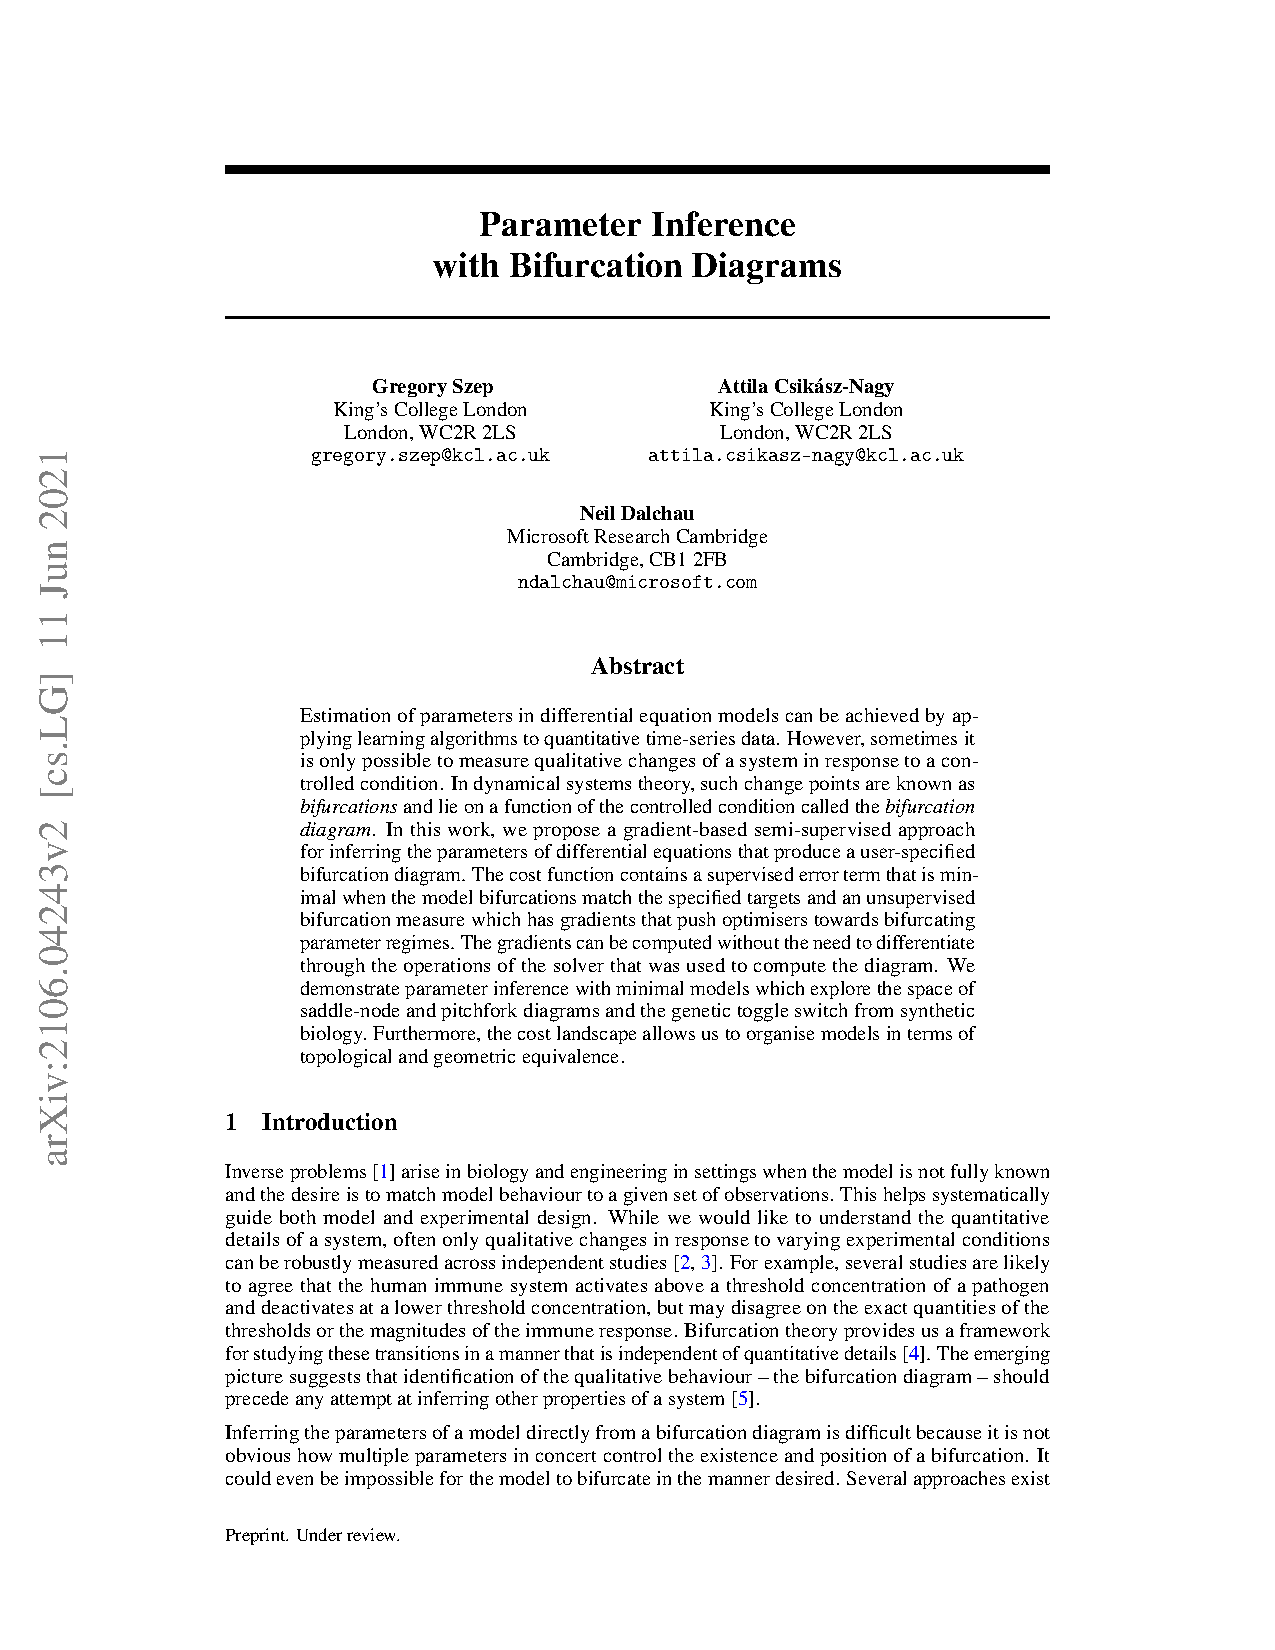
\includepdf[pages=-, offset=75 -75, addtotoc={
        1,section,1,Introduction,section:introduction,
        2,subsection,2,Preliminaries,preliminaries,
        4,section,1,Proposed Method,section:method,
        4,subsection,2,Semi-supervised Cost Function,cost,
        5,subsection,2,Differentiating the semi-supervised cost function,derivatives,
        6,section,1,Experiments \& Results,section:results,
        6,subsection,2,Minimal Models,minimal,
        6,subsection,2,Genetic Toggle Switch,genetic,
        7,subsection,2,Complexity,complexity,
        9,section,1,Conclusion \& Broader Impact,section:impact,
        9,section,1,Acknowledgements,section:acknowledgements,
        12,section,1,Appendix,section:appendix,
        12,subsection,2,Bifurcation Diagrams as Tangent Fields,tangent-fields,
        13,subsection,2,Conditions for Bifurcations,conditions,
        14,subsection,2,Leibniz Rule for Space Curves,leibniz-rule},
    addtolist={
        3, figure, {Illustration of bifurcation diagrams for minimal models of bifurcations. A. Saddle-node bifurcations arise for $\rates(u,p) = p + \theta_{1}u+\theta_{2}u^3$ when $\theta = (\frac{5}{2},-1)$. B. Pitchfork bifurcations arise for $\rates(u,p) = \theta_{1} + p u+\theta_{2}u^3$ when $\theta=(\frac{1}{2},-1)$. Targets are illustrated by light yellow vertical lines. Bifurcation curves are shown as solid blue and red lines, with lighter shades indicating the determinant crossing zero at locations $\predictions(\theta)$ giving rise to unstable solutions.}, figure:minimal-models,
        4, figure, {Bifurcation measure $\measure(s)$ and determinant $\Det$ along the arclength $s$ of two different bifurcation curves demonstrating how maximising the measure along the curve maintains the existing bifurcation marked by a circle, while encouraging new bifurcations marked by stars.}, figure:measure,
        7, figure, {Saddle-node $\rates(u,p) = p + \theta_{1}u+\theta_{2}u^3$ and pitchfork $\rates(u,p) = \theta_{1} + u p +\theta_{2}u^3$ optimised with respect to $\theta$ so that predicted bifurcations $\predictions(\theta)$ match targets $\targets$ in control condition $p$. The right panel shows bifurcations diagrams for the three optimal $\theta^*$ marked by stars on the left panel. The optimisation trajectories in white follow the gradient of the cost, approaching the black lines of global minima in the left panel}, figure:minimal-models:results,
        8, figure, {Bifurcation inference for the two-state model (11). A. Optimal parameter estimates $\theta^*$ for the targets $\targets=\{4,5\}$ reveal two clusters of qualitatively different regimes: mutual activation ($a_1 < 1$; cluster 1) and mutual inhibition ($a_1 > 1$; cluster 2). B. Example bifurcation diagrams indicate positively and negatively correlated dependencies between the two model states, as a function of the control condition.}, figure:two-state-optima,
        8, figure, {Complexity scaling of calculating the gradient of the cost function. Calculations were performed on an Intel Core i7-6700HQ CPU @ 2.60GHz x 8 without GPU acceleration}, figure:scaling
}]{publications/bifurcation-inference.pdf}